\documentclass[fontsize=14pt,svgnames]{scrreprt}
\usepackage{style}
\begin{document}
	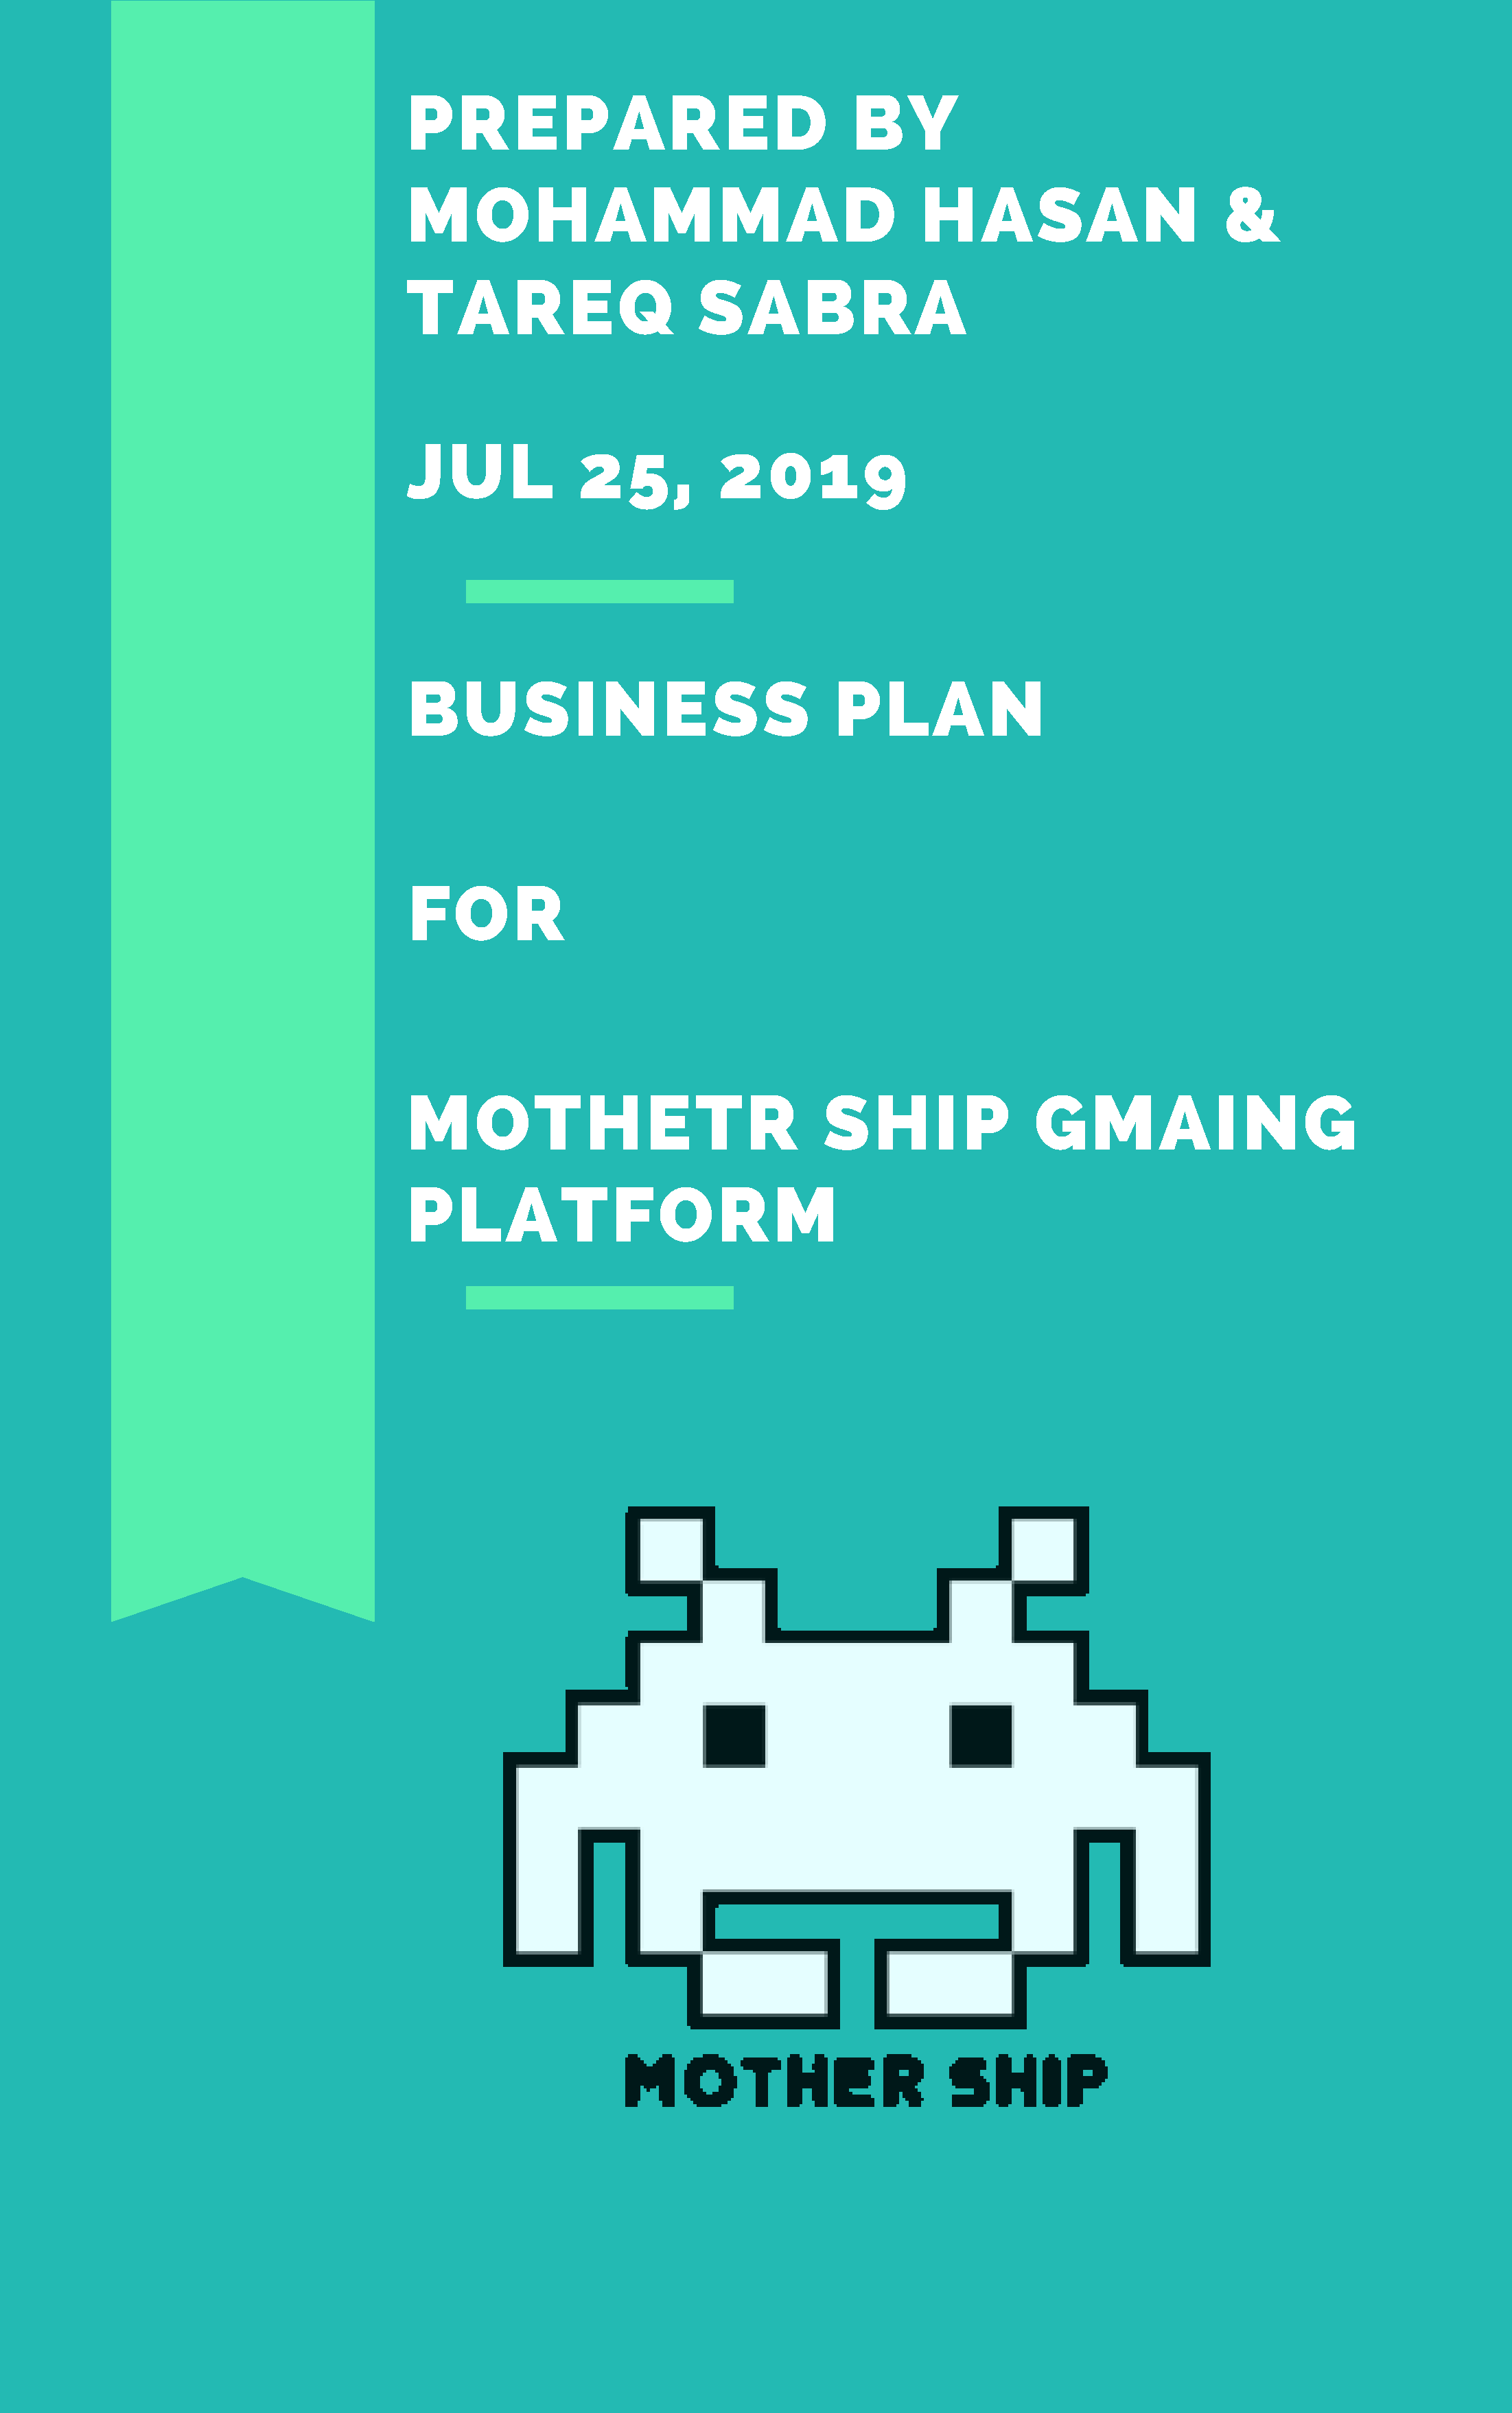
\includepdf[width=21cm,height=29.7cm]{PDFS/BPTitlePage.pdf} 
\tableofcontents
\listoftables
\listoffigures
%\clearpage
\chapter{Executive Summary}
The mother ship company is a game distribution platform that aims to help Arab developers to find a suitable place and market to sell their products and get in-time feedback.
\par This company is The first of its kind in Palestine and with almost no rivals  in the Arab world  is expected to make a huge success within few years of business due  to many factors such as the growing power of game industry and the increasing market share of Arab countries in the international game market.
\par The main sources of profit for this business are gamers monthly subscription fees ,fees on publishing game titles, game sales revenue cuts and ads advertisement.It's expected that this business will get to the break even point within a year and a month and a half  of business.
\par Our target customers are Arab game and independent developers, advertisers and gamers.Those customers can access our services throw our website and their products will be distributed throw the website as well.
\par We’ll ensure the quality of products sold on our website as a part of our policy of making us different from our competitors with the ability to refund products within certain conditions and reasons  and having a reliable support team to ensure maximum customer satisfaction and trust. 
\par The company is registered as partnership company and is owned by Mohammad Hasan and Tareq Sabra which share the responsibilities for the company and have dividends shared evenly between them.
\par The company shall be located in the center of Nablus and will require a startup cost of about 3000\$.The company has a small set of fixed assets which are the database server and a 2 desktops.
\par In the three years of the company start,only Tareq and Mohammad will work in it and shall do all the managerial activities in-addition to the other operational activities such as database maintenance and providing web customer services in-addition to company advertisement and promotion operations.   
\par Our company vision be one of the best Arabic game distribution platform and be the best home for Arabic independent developers.

\chapter{Company Description}
Our company is named "The Mother Ship", it will be located in the center of Nablus in Palestine and will be owned by Tareq Sabra and Mohammad Hasan. The company will serve Arabic developers and gamers with user friendly gaming platform were the developer can easily sell his product and get in-time feedback from the customers.
\par The start-up of this company is going to be funded partly (around 10\%) by its owners and hopefully, the rest of the fund will come from organizations who read this plan and find an opportunity in incubating us as entrepreneurs.  
\section{Mission \& Vision}
Our company mission is to help Arabic developers by publishing their games 
and providing an easy, user friendly market to sell these games in and give them in-time feedback from real customers and gamers to improve their games and skills.
\par Our vision is to be one of the best Arabic game distribution platform and be the best home for Arabic independent developers.
\section{Products and Services}
The company  has its own online website and will provide its customers with three main services:
\begin{itemize}
\item Subscribed gamers will be able to download and play the company's platform provided games.
\item Developers who've registered in the company website will be able to publish their games on the website which can be sold to the gamers who in turns enhance developers returns and give them technical feedback on their work.
\item Advertisers who've contracted with the company will be able to advertise their products and services on the company website and promotional emails.
\end{itemize}
\section{Ownership}
The Mother Ship company will be owned by Tareq Sabra and Mohammad Hasan.\par Tareq is a computer engineer with one year experience in web design and has experience in developing game support sites.Tareq will held the position of General Manager of this company.
\par Mohammad Hasan is a computer engineer with over 2 years of experience in databases and platform administration and will be positioned as the Assistant Manager of this company.
\section{Legal Form}
The Mother Ship company will be registered in Companies Registration Department at the Palestinian Ministry of National Economy as a partnership organization and will be owned by Tareq Sabra and Mohammad Hasan.
\section{Location and Facilities}
\par The company will take a place in the center of Nablus in a one-room \footnote{The  owner of this studio advertise it on \url{https://shobiddak.com/houses}.} (studio) which comes already furnished and will cost about \SI{185}[\$]{} per month as a rent.   
\par This location of the company make it easy for our employees to reach and is enough for the start-up.Though,in future another place shall be found as the company evolves and get bigger. 
\chapter{Market/Industry \& Competitor Analysis}
The Member Ship company is going to provide games from its registered developers to its subscribed gamers and thus our targeted market is both the game
market and the game distribution platforms market.
\section{Market study}
The video game industry has grown really fast over the years, its market reached \SI{78.61}[\$]{B} in 2017 and is expected to be worth over \SI{90}[\$]{B} by 2020 with a growth rate of over 18\%.
\begin{figure}[H]
\centering
  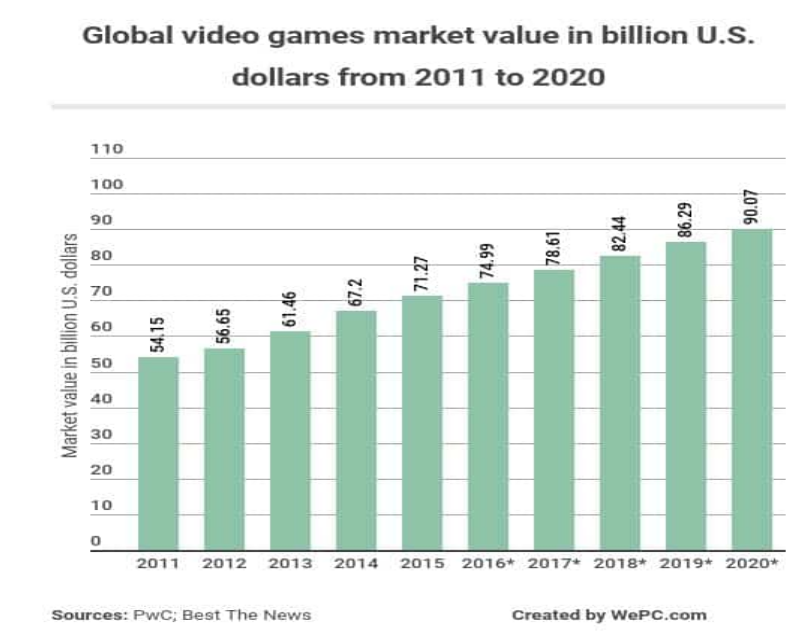
\includegraphics[width=\linewidth,height=15cm]{Diagrams/video-games-market-value.png}
    \caption{\small{Video-Games market.\protect\footnotemark}}
  \label{fig:1}
\end{figure}
\footnotetext{Taken from \url{https://www.statista.com/statistics/547025/steam-game-sales-revenue.}}
\par As game industry grows there is an increasing need for online gaming platforms
where developers can distribute their games without the obstacles of intermediaries and increase their profits.
\par When taking about gaming distribution platforms Steam is the first one in this industry with an active user base (\SI{125}[]{M}) that rivals the combined user bases of the current console generation (\SI{150}[]{M}) which make it dominates the market.
Steam's share of the market grew from \SI{3.5}[\$]{B} in 2016 to \SI{4.3}[\$]{B} in 2017 with a growth rate of about 22\% .
\begin{figure}[H]
\centering
  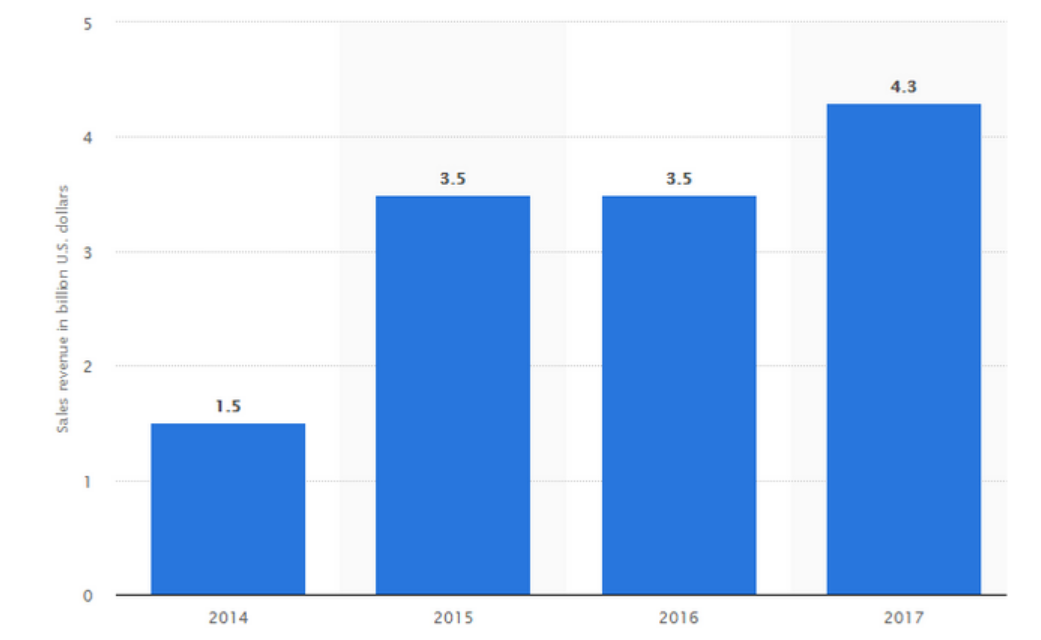
\includegraphics[width=\linewidth]{Diagrams/steam-market.png}
    \caption{\small{Steam market\protect\footnotemark.}}
  \label{fig:1}
\end{figure}
\footnotetext{Taken from \url{https://www.wepc.com/news/video-game-statistics}.}
\par Nintendo, Sony and Microsoft are considered the best game-selling companies
which monopolize 85\% of the game global market share, while China is the
largest consumer market for these products by nearly 20\%.In the Arab world,
the Gulf Arab countries occupy the highest rates of consumption of electronic
games, especially Saudi Arabia, about 28\% of the Arab market.\footnote{According to \url{http://tiny.cc/mk3caz}.}
\par About two-thirds in Saudi Arabia and the UAE play video games (65\% and
63\%, respectively), while closer to three in ten in Qatar and Egypt do so (33\% and 29\%, respectively). Four in ten play in Lebanon, and only a quarter play video games in Tunisia.
\par Relatively few gamers play video games on a daily basis (14\%), although those
under 25 are more likely to do so (29\%).The typical (median) time gamers spend
playing video games is five hours each week.\footnote{According to \url{http://www.mideastmedia.org/survey/2014/video-games/popularity-of-video-games-and-time-spen
html}.}
\par All of these numbers indicate how strong the game-industry market is and it
gets stronger by the time working with other industries like the hardware industry
and many others, and all the signs indicate that the future for this industry will
only become better and stronger.
\par Indie games are games made by individuals developers or small studios.They grow largely over the years with the existence of new and free game engines such as unity which makes it easy for small developers to produce quality games.Our company aims at targeting this slice of developers to publish their work on the company website.
\par Steam indie games has grown and the estimated number of indie games are about \SI{22}[]{K} and with market share of about 5\% which give us an estimate of a market size with \SI{130}[]{K} unit of games and with an avg price of \SI{7}[\$]{} per each unit, the size of the targeted market is about \SI{910}[\$]{K}.

\section{Competitors Analysis}
To prove that this investment is feasible and that we have an advantage against
possible competitors threats, the 5 forces model(porters model) is applied.
\subsection{Rivilary Among Existing Firms: Medium Pressure}
In this industry Steam is the dominant but it will have a direct competition with Epic which owns many games in the market and is going to launch its own online engine which include its made games and will be welcoming for other independent publishers.
\par Other competitors in the market are Unity,Bulizard,GOG and Gamersgate but they have less effects on the industry.
\par The Arabian and Palestinian game publishing industry  almost has no competitors 
where there's no companies  specialized in supporting Arab game developers or publishing their games online or selling them.
\subsection{Threat of Substitutes: Low Pressure}
Independent publishers can publish their games to Steam and Epic.Developers and publishers pay Steam 30\% for every game sale on the platform whereas they will pay Epic Games just 12\%.
\par Arabic independent game developers find it really hard to sell or publish their games on these platforms for reasons like:
\begin{itemize}
\item There's no actual  international fan base for Arabic developed games. 
\item There is no trust in the quality of Arabic developed games and therefore no one up votes the game in these stores. 
\end{itemize}
\par Our company aims at providing a welcoming environment for developers were they can easily share their games with low revenue cuts and thus make it an advantage against going for other substitutes.
\subsection{Bargaining Power of Buyers: High Pressure}
 Video games have a very high purchases.Consumers are looking forward to play a high quality games and with low costs and thus they tend to go to big games rather than games developed by independent suppliers and these games are found on distribution like Steam,Epic and Ubisoft.
 \par Though this have a high risk on our company but a turn over on this threat would be to not only bring Arabic independent games but also to bring trending games to the company platforms along with special offers at the lowest prices possible.    
\subsection{Bargaining Power of Suppliers: Medium Pressure} 
Arabic independent developers find it hard to distribute their games to big platforms because they have to pay (relatively high) fixed costs to these companies before they even begin to get revenues from their games for instance Steam require their publishers to pay \SI{100}[\$]{} which is considered high and risky for Arabic small developers.Also, big game distribution like Steam will keep cutting a percent (around 30\%) for each payment of game developed by its customers.
\par Our company aims at incubating these small developers by putting a small and affordable costs on publishing games and get a low percent (8\%) on each sold game and thus gaining publishers loyalty and decreasing the probability of switching to another company.     
\subsection{Threats of New Entrants: Low Pressure}
Big distribution like Steam has many competitors since their suppliers are a very big company like Ubisoft,Epic and CD-Project who can at moment build their own distribution platforms.On the other hand,the Arab world is witnessing stagnation in the huge gaming industry and tends to invest in small non-risky ones and thus it has no native platforms for its publishers.
\par Thus the risk of new entrants from new Arab competitors is very low which give us a first-mover advantage toward this industry.
\section{Competitive Advantage}
There are no companies specialized in supporting Arab game developers,publishing
their games online or selling them and our company will aim at diminish such
gaps by being the first-mover toward this business in the Arab world.
\par Big platforms such as Steam doesn’t support Arab currencies and thus make
it hard for Arab to buy the product,Players in the Middle East The interest
of electronic stores in Arabic currencies in their shops so that we can buy in
our official currency without transfer fees are collected over the amount of the
game when you buy.Our company will support almost all the Arab Currencies
to diminish this gap.
\section{Future threats} 
There are threats that may face this company as it grows.The most affecting threats are the illegal distribution of the games done by hackers ,but we would note that this threat may only occur in the far future when the company has an international reputation and its games are highly requested and can be faced throw services like Denuvo.Our defensive strategy for this threat is to make deals with online services which makes the website games more secure and hard to break. 
\chapter{Marketing Plan}
Our business aims to encourage Arab game developers and give them the ability to sell their products in local and global markets  by giving them and their games the attention and customer feedback they need.
\section{Key Performance Indicators (KPI) }
\par The company focuses on the following points to measure its performance:
\begin{itemize}
\item Number of times our web page is viewed and visited.
\item Number of gamers who've subscribed in our website.
\item Number of developers who've registered in our website.
\item Number of advertiser who've contracted or are considering a contract with our company to advertise on our website.
\item Number of games sold through our website.
\end{itemize}
\section{Customers Personas}
The company aims at attracting Arab game developers who make quality games and want to sell and increase their profit from them.
\par We also aim at attracting customers and investors who are interested in Arab-developed games, those customers could be local customers (from within Palestine) or international (from nearby countries such as Gulf-countries,Egypt and Tunisia).
\par We also aim at attracting a third personas which is advertisers who want to improve their businesses by targeting their ads to gamers and developers in our environment.  
\section{Marketing Objectives}
The company considers the following marketing objectives
\begin{itemize}
\item  To break even within a year and a quarter of business.
\item To dominate the Arab world game industry and become the $1^{st}$ distributor of Arab games within 5 years of time
\item To expand and start competing world-wide.
\item To have an international market share within 10-15 years of business.
\end{itemize}
\section{Marketing Mix}
In this section, we consider the 4 marketing mix to satisfy the needs and desires of consumers whether they are gamers,developers or advertisers.
\subsection{Product}
\par The quality level of products distributed by developers are important so for a game to be sold by our company and exist on our website it has to meet up with the following quality standards:
\begin{itemize}
\item The game has to work properly and reported bugs shall be solved by the developer as soon as possible. 
\item The game should be compatible with the OS's that it is developed for.
\item The game should has a content that is reasonable with its sold cost.
\item The game should meet our community standards and being suitable for the genre it's being sold or advertised for.
\end{itemize}
\par  As part of the company design and styles,game developers have to declare what language or engine is used to design their games and what  genre it's directed to.
\par The website distributed games are guaranteed to have developer support and a satisfying level of quality which enhances the company features.
\par As a branding strategy, games will have their developer logo as the game makers and our logo as the game distributors and will be registered in both our name and the developer's name.
\par The size of games distributed in the platform is not limited and depends on the game contents and technology.
\par As part of our company sale strategies,we provide our customers with fast reliable support and a new market to sell their games in and advertise their products. 
\par The company ensure a full refund on its sold games as part of its warranty for the customers and this may occur in cases like:
\begin{itemize}
\item The game didn't work due to a developer error.
\item The game was different from its description.
\end{itemize}
\subsection{Pricing}
The company aims when determining prices is to make reasonable profit through the developer subscription,the small cut percentage on the sold games revenue and through payments for advertising activities. 
\par The game price elasticity is affected by the change in demand of a certain game which affect its popularity causing us to reduce its price and  make offers and deals on it.On the other hand, if the demand increases the price of the game wont change ( won't become less).
\par As a pricing method strategy,the price of games is determined by its content,how much time it took to make and the resources where used in developing it and thus any game with price that doesn't reflect its content and quality won't be distributed in our website.
\subsection{Place}
Our customers can access our services through the company website where they can subscribe and download games or distribute it or contract with the company to advertise their products.
\par The only way to get our services is through our website and this strategy is adopted to diminish costs on contracts with agents to distribute our products and to reach the largest possible segment of potential customers.
\subsection{Promotion} 
Social media has proven to be very effective in promoting products and bring in customers.This method of promotion is considered cheap and effective for start-ups and thus at the beginning,we plan to get to our customers through social media advertisement.
\par After making a name and building a reputation for the company,we plan to use Google targeted ads to advertise the website and the company to different developers,gamers and advertisers.
\chapter{Operation Plan}   
The location of the project has been chosen so that it is close to the staff and easy to reach.It has also been taken into account that the cost of rent should be as low as possible so that the impact of fixed costs is low.
\par The project is located in the center of Nablus in a small studio room with a rent,thus ensuring lower transportation costs for the staff.
\par The site is furnished and ready for use, but needs to be supplied with water, electricity and internet from the company's expenses.
\par For the company to start,it needs a server to do the following:
\begin{itemize}
\item Storing the databases of the developers games.
\item Storing financial transactions and operations.
\item Storing employees information and salaries \& customers transactions,subscription plans and their website tracks.  
\end{itemize}  
\par The company needs two computers for both the cooperator of this company which will use it for the following activities:
\begin{itemize}
\item Monitoring the work in the company and its employees.
\item Monitoring financial transactions and pay the company bills.
\item Paying the employees salaries and make weekly operation plan.
\item Database management and maintenance.
\item Website tracking,maintenance and security.
\item Reply to business and customers messages. 
\end{itemize}
The company also needs a server to host the website on it.We are going to use the  Blue Host service as it serve a low costs on web hosting with enough space and free domain for considerable time and it offers automated backup for the website thus remove the part of the overhead on the company.
\par The website also needs to be promoted and we plan to do that using social media both by putting latest products promotion in the company social pages and by taking low cost offers these social medias.
\par The project initially needs an employee who can deal with customers and support them.That the employee should be aware of the efficient methods in promoting digital products through social medias and video-sharing websites like YouTube.Also he should have the skills of fulfilling customer needed services,communicate with them and hear their complaints and suggestions through our website,social pages and official e-mails.
\par The nature the work requires our employees to bring their personal computers with them to do the different company activities and by applying this strategy we reduce the overhead of tool expenses on the company.
\chapter{Management \& Organization}
In order to start the work, it needs human resources managed and be able to bear the responsibilities assigned to it and work for the company success and promote it.
\par For the company to succeed, it needs structural organization.\par There have to be a CEO who manages the organizations overall goals,strategy, and operating policies and be responsible for the entire enterprise.\par There have to be a general manager responsible about the department different functionality.\par There have to be a financial and marketing managers to get consumers to buy the company's products and to deal with the company's financial resources.\par There have to be a human resource manager responsible for recruiting and selection of the employees.
\section{Human Resources}
When the company start-ups it needs 3 persons to operate it and share all the responsibilities of all units in the structural organization mentioned above.
\begin{itemize}
\item Mohammad Hasan will be one of the co-founder of the company and will take the responsibilities of maintenance and organization of the company databases.He will be responsible of tracking employees works and assigning them weekly plans.He will also be responsible for the financial of the company.
\item Tareq Sabra is also one of the co-founders and will be responsible for the website maintenance and debugging and will add any demanded feature for it.He will also be responsible for replying business messages and will be in charge of tracking the company devices.
\item The third person is an employee which will be selected by Mohammad and will be responsible for promoting the company's website and deal with customers and will act as the support team for our company.    
\end{itemize}
\par Working together, all the functionalities required by the different managerial levels should be fulfilled.
\chapter{Financial Statements}
In this section, we will present an estimate of the financial statements for the three years following the commencement of the project.These estimates are based on the market analysis done previously in the report and based on the customary costs in the Palestinian market.
\par The company needs a place where it can put its database servers and where the employees will meet.The rent of the small-furnished studio will have a fixed cost of \SI{1220}[\$]{K} per year, other fixed costs are the cost of the database server (\SI{700}[\$]{}) and the cost of two desktop as there will be two employees (\SI{170}[\$]{}).Also,the company is registered as a partnership company which costs \SI{130}[\$]{}. 
\par Variable costs are spent on web hosting,advertisement,salaries and transportation.Web hosting will initially cost 10\$ per each month and we will spent 100\$ on advertisement (15\$ will go as a Facebook web-page advertising and the rest will go in other forms of advertising).\par The owners of this company will initially be the only employees and each of them will have a salary of \SI{570}[\$]{} per each month.The employees lives in nearby villages near Nablus and hence a transportation of \SI{2.28}[\$]{} per day for 5 days a week (working days).
\par The revenue drivers of the company depend on three main sources described as follows:
\begin{itemize}
\item Subscription fees on customers who download and play the platform games this subscription will cost the customer \SI{5}[\$]{} for each month and shall be payed at the start of each month.
\item Every published game requires its developer to pay \SI{5}[\$]{} before it launches on the company platform and there's a revenue cut of 10\% on each sold game.
\item Contracts with advertisers who want to advertise their products on the company websites apps and emails,this have an average of  \SI{3}[\$]{} every month per each customer.     
\end{itemize}
\par From the revenue drivers mentioned above,the revenue of the company per each year is given by the following multivariate function:
\begin{equation}
R(P,G_{new},C_{avg},D_{avg},A)=60P+5G_{new}+0.1C_{avg}D_{avg}+36A\;\$
\end{equation}
where:
\begin{conditions}
 P     &   Number of players in this year \\
 G_{new}     &  Number of new games published on the website in this year \\   
 C_{avg} &  Average price of a game in this year \\
 D_{avg} & Average game downloaded (purchased) this year \\
 A & Number of advertisers in this year 
\end{conditions} 
\par The depreciation year for the server and the desktops is 5 years and all the tables where filled with time value of the money already discounted. 
\section{Performa Income Statement}
The performa income statement for the next three years is shown in the following table:
% Please add the following required packages to your document preamble:
% \usepackage[table,xcdraw]{xcolor}
% If you use beamer only pass "xcolor=table" option, i.e. \documentclass[xcolor=table]{beamer}
\begin{table}[!H]
\begin{tabular}{|l|l|l|l|l|}
\hline
\rowcolor[HTML]{23BAB3} 
\multicolumn{2}{|c|}{\cellcolor[HTML]{23BAB3}\textbf{Income Statement}}    & \multicolumn{1}{c|}{\cellcolor[HTML]{23BAB3}\textbf{1st Fiscal Year}} & \multicolumn{1}{c|}{\cellcolor[HTML]{23BAB3}\textbf{2nd Fiscal Year}} & \multicolumn{1}{c|}{\cellcolor[HTML]{23BAB3}\textbf{3rd Fiscal Year}} \\ \hline
\rowcolor[HTML]{529BB6} 
\multicolumn{5}{|c|}{\cellcolor[HTML]{529BB6}\textbf{Revenues}}                                                                                                                                                                                                                                    \\ \hline
\multicolumn{2}{|l|}{\cellcolor[HTML]{23BAB3}Subscription Fees}            & 12360                                                                 & 21600                                                                 & 36000                                                                 \\ \hline
\multicolumn{2}{|l|}{\cellcolor[HTML]{23BAB3}Game Publish Fees}            & 75                                                                    & 100                                                                   & 150                                                                   \\ \hline
\multicolumn{2}{|l|}{\cellcolor[HTML]{23BAB3}Game Revenue Cuts}            & 70                                                                    & 187.5                                                                 & 300                                                                   \\ \hline
\multicolumn{2}{|l|}{\cellcolor[HTML]{23BAB3}Advertising Fees}             & 3600                                                                  & 5400                                                                  & 7200                                                                  \\ \hline
\multicolumn{2}{|l|}{\cellcolor[HTML]{23BAB3}\textbf{Ttoal Revenue}}       & \textbf{16105}                                                        & \textbf{27287.5}                                                      & \textbf{43650}                                                        \\ \hline
\rowcolor[HTML]{529BB6} 
\multicolumn{5}{|c|}{\cellcolor[HTML]{529BB6}\textbf{Variable Cost}}                                                                                                                                                                                                                               \\ \hline
\multicolumn{2}{|l|}{\cellcolor[HTML]{23BAB3}Desktops}                     & 170                                                                   & 0                                                                     & 0                                                                     \\ \hline
\multicolumn{2}{|l|}{\cellcolor[HTML]{23BAB3}Servers}                      & 700                                                                   & 0                                                                     & 0                                                                     \\ \hline
\multicolumn{2}{|l|}{\cellcolor[HTML]{23BAB3}Company Registration}         & 130                                                                   & 0                                                                     & 0                                                                     \\ \hline
\multicolumn{2}{|l|}{\cellcolor[HTML]{23BAB3}Depreciation}                 & 174                                                                   & 174                                                                   & 174                                                                   \\ \hline
\multicolumn{2}{|l|}{\cellcolor[HTML]{23BAB3}Rent}                         & 1220                                                                  & 1220                                                                  & 1220                                                                  \\ \hline
\multicolumn{2}{|l|}{\cellcolor[HTML]{23BAB3}\textbf{Total Fixed Cost}}    & \textbf{2394}                                                         & \textbf{1394}                                                         & \textbf{1394}                                                         \\ \hline
\rowcolor[HTML]{529BB6} 
\multicolumn{5}{|c|}{\cellcolor[HTML]{529BB6}\textbf{Variable Cost}}                                                                                                                                                                                                                               \\ \hline
\multicolumn{2}{|l|}{\cellcolor[HTML]{23BAB3}Web Hosting}                  & 120                                                                   & 150                                                                   & 200                                                                   \\ \hline
\multicolumn{2}{|l|}{\cellcolor[HTML]{23BAB3}Avertisement}                 & 100                                                                   & 700                                                                   & 2000                                                                  \\ \hline
\multicolumn{2}{|l|}{\cellcolor[HTML]{23BAB3}Salaries}                     & 13680                                                                 & 13920                                                                 & 14160                                                                 \\ \hline
\multicolumn{2}{|l|}{\cellcolor[HTML]{23BAB3}Transportation}               & 1186                                                                  & 1186                                                                  & 1186                                                                  \\ \hline
\multicolumn{2}{|l|}{\cellcolor[HTML]{23BAB3}Utilities}                    & 548                                                                   & 548                                                                   & 548                                                                   \\ \hline
\multicolumn{2}{|l|}{\cellcolor[HTML]{23BAB3}\textbf{Total Variable Cost}} & \textbf{15634}                                                        & \textbf{16504}                                                        & \textbf{18094}                                                        \\ \hline
\multicolumn{2}{|l|}{\cellcolor[HTML]{23BAB3}\textbf{Profit/Loss}}         & \textbf{-1923}                                                        & \textbf{9389.5}                                                       & \textbf{24162}                                                        \\ \hline
\multicolumn{2}{|l|}{\cellcolor[HTML]{23BAB3}Income Tax}                   & 15\%                                                                  & 15\%                                                                  & 15\%                                                                  \\ \hline
\multicolumn{2}{|l|}{\cellcolor[HTML]{23BAB3}\textbf{Net Income}}          & \textbf{-1923}                                                        & \textbf{7981.075}                                                     & \textbf{20537.7}                                                      \\ \hline
\end{tabular}
\end{table}

\par The table above showed a projected revenues for subscription fees,game publish fees,game cuts and advertising fees.These revenues are based on the market analysis done before which shows share of games,users and developers and which can be found at \url{https://www.wepc.com/news/video-game-statistics/}.The projected qunatity of each revenue drivers were estimated and plugged in the revenue equation mentioned earlier and then filled within the statement table.
\par As seen from the table the profit to revenue ratio are increasing as the company ages with percents of -15\%,43.46\% and 55.35\% respectively which shows a good potential in the market.
\par The income tax rate on partnership companies is taken from the following site \url{https://www.pipa.ps/ar_page.php?id=1b102fy1773615Y1b102f}. 
\section{Performa Cash Flow Satatement}
It has to be noticed that the services bought on the company website goes immediately to the company's cash so there are no accounts receivable,nor from subscribed gamers and neither from registered developers or advertisers.
\par It also has to be noticed that the company pays all its obligations from rent,utilities,web hosting,etc in cash immediately so there are no payable accounts,bonds or notes.
\par The performa cash flow statement for the next three years is shown in the following table:
% Please add the following required packages to your document preamble:
% \usepackage[table,xcdraw]{xcolor}
% If you use beamer only pass "xcolor=table" option, i.e. \documentclass[xcolor=table]{beamer}
\begin{table}[!H]
\begin{tabular}{|c|c|c|c|c|}
\hline
\rowcolor[HTML]{23BAB3} 
\textbf{\begin{tabular}[c]{@{}c@{}}Balance \\ Sheet\end{tabular}} & \multicolumn{2}{c|}{\cellcolor[HTML]{23BAB3}\textbf{\begin{tabular}[c]{@{}c@{}}1st Fiscal\\ Year\end{tabular}}} & \textbf{\begin{tabular}[c]{@{}c@{}}2nd Fiscal\\ Year\end{tabular}} & \textbf{\begin{tabular}[c]{@{}c@{}}3rd Fiscal\\ Year\end{tabular}} \\ \hline
\rowcolor[HTML]{529BB6} 
\multicolumn{5}{|c|}{\cellcolor[HTML]{529BB6}\textbf{Inflow Cash}}                                                                                                                                                                                                                                                            \\ \hline
\multicolumn{2}{|c|}{\cellcolor[HTML]{23BAB3}Revenue Cash}                                                          & 16105                                                         & 27287.5                                                            & 43650                                                              \\ \hline
\multicolumn{2}{|c|}{\cellcolor[HTML]{23BAB3}New Personal Cash}                                                     & 100                                                           & 0                                                                  & 0                                                                  \\ \hline
\multicolumn{2}{|c|}{\cellcolor[HTML]{23BAB3}Previous Fiscal Cash}                                                  & 0                                                             & 1174                                                               & 4079.075                                                           \\ \hline
\multicolumn{2}{|c|}{\cellcolor[HTML]{23BAB3}Loan Cash}                                                             & 2823                                                          & 0                                                                  & 0                                                                  \\ \hline
\multicolumn{2}{|c|}{\cellcolor[HTML]{23BAB3}\textbf{Ttoal Cash Inflow}}                                            & \textbf{19028}                                                & \textbf{28461.5}                                                   & \textbf{47729.075}                                                 \\ \hline
\rowcolor[HTML]{529BB6} 
\multicolumn{5}{|c|}{\cellcolor[HTML]{529BB6}\textbf{Outflow Cash}}                                                                                                                                                                                                                                                           \\ \hline
\multicolumn{2}{|c|}{\cellcolor[HTML]{23BAB3}Investment in Servers and Desktops}                                    & 870                                                           & 0                                                                  & 0                                                                  \\ \hline
\multicolumn{2}{|c|}{\cellcolor[HTML]{23BAB3}Registration}                                                          & 130                                                           & 0                                                                  & 0                                                                  \\ \hline
\multicolumn{2}{|c|}{\cellcolor[HTML]{23BAB3}Hosting and Advertisment}                                              & 220                                                           & 850                                                                & 2200                                                               \\ \hline
\multicolumn{2}{|c|}{\cellcolor[HTML]{23BAB3}Salaries and Transportation}                                           & 14866                                                         & 15106                                                              & 15346                                                              \\ \hline
\multicolumn{2}{|c|}{\cellcolor[HTML]{23BAB3}Utilities and Rent}                                                    & 1768                                                          & 1768                                                               & 1768                                                               \\ \hline
\multicolumn{2}{|c|}{\cellcolor[HTML]{23BAB3}Loan Payment}                                                          & 0                                                             & 250                                                                & 1000                                                               \\ \hline
\multicolumn{2}{|c|}{\cellcolor[HTML]{23BAB3}Other expenses (Taxes)}                                                & 0                                                             & 1408.425                                                           & 3080.655                                                           \\ \hline
\multicolumn{2}{|c|}{\cellcolor[HTML]{23BAB3}Divedends}                                                             & 0                                                             & 5000                                                               & 15000                                                              \\ \hline
\multicolumn{2}{|c|}{\cellcolor[HTML]{23BAB3}\textbf{Total Cash Outflow}}                                           & \textbf{17854}                                                & \textbf{24382.425}                                                 & \textbf{38394.655}                                                 \\ \hline
\multicolumn{2}{|c|}{\cellcolor[HTML]{23BAB3}\textbf{Net Cash}}                                                     & \textbf{1174}                                                 & \textbf{4079.075}                                                  & \textbf{9334.42}                                                   \\ \hline
\end{tabular}
\end{table}

\section{Performa Balancesheet}
The balance sheet for the first three years of the company are described in the following table: 
% Please add the following required packages to your document preamble:
% \usepackage[table,xcdraw]{xcolor}
% If you use beamer only pass "xcolor=table" option, i.e. \documentclass[xcolor=table]{beamer}
\begin{table}[!H]
\begin{tabular}{|
>{\columncolor[HTML]{23BAB3}}c |c|l|c|c|}
\hline
\textbf{\begin{tabular}[c]{@{}c@{}}Balance\\ Sheet\end{tabular}} & \multicolumn{2}{c|}{\cellcolor[HTML]{23BAB3}\textbf{\begin{tabular}[c]{@{}c@{}}1st Fiscal\\ Year\end{tabular}}} & \cellcolor[HTML]{23BAB3}\textbf{\begin{tabular}[c]{@{}c@{}}2nd Fiscal\\ Year\end{tabular}} & \cellcolor[HTML]{23BAB3}\textbf{\begin{tabular}[c]{@{}c@{}}3rd Fiscal\\ Year\end{tabular}} \\ \hline
\multicolumn{5}{|c|}{\cellcolor[HTML]{529BB6}\textbf{Assets}}                                                                                                                                                                                                                                                                                                                \\ \hline
Non Current Assets                                               & \multicolumn{2}{c|}{826}                                                                                        & 652                                                                                        & 478                                                                                        \\ \hline
Cash                                                             & \multicolumn{2}{c|}{1174}                                                                                       & 4079.075                                                                                   & 9334.42                                                                                    \\ \hline
Inventory \& Recievables                                         & \multicolumn{2}{c|}{0}                                                                                          & 0                                                                                          & 0                                                                                          \\ \hline
\textbf{Ttoal Assets}                                            & \multicolumn{2}{c|}{{\color[HTML]{FD6864} \textbf{2000}}}                                                       & {\color[HTML]{CE6301} \textbf{4731.075}}                                                   & {\color[HTML]{963400} \textbf{10267.42}}                                                   \\ \hline
\multicolumn{5}{|c|}{\cellcolor[HTML]{529BB6}\textbf{Liabilities and Owner’s Equity}}                                                                                                                                                                                                                                                                                        \\ \hline
Owner’s Equity                                                   & \multicolumn{2}{c|}{100}                                                                                        & 100                                                                                        & 100                                                                                        \\ \hline
Loans                                                            & \multicolumn{2}{c|}{2823}                                                                                       & 2573                                                                                       & 1573                                                                                       \\ \hline
Retained Eearnings                                               & \multicolumn{2}{c|}{-923}                                                                                       & 2058.075                                                                                   & 8594.42                                                                                    \\ \hline
\textbf{Total of Liabilities and Equities}                       & \multicolumn{2}{c|}{{\color[HTML]{FD6864} \textbf{2000}}}                                                       & {\color[HTML]{CE6301} \textbf{4731.075}}                                                   & {\color[HTML]{963400} \textbf{10267.42}}                                                   \\ \hline
\end{tabular}
\end{table}


\section{Breakeven Analysis}
Since the revenue from the services are given by multivariate quantities,we choose to make the breakeven analaysis by plotting the revenues and total costs as a function of time.
\par The following graph shows the breakeven point between total revenues and total costs:
\begin{figure}[H]
\centering
  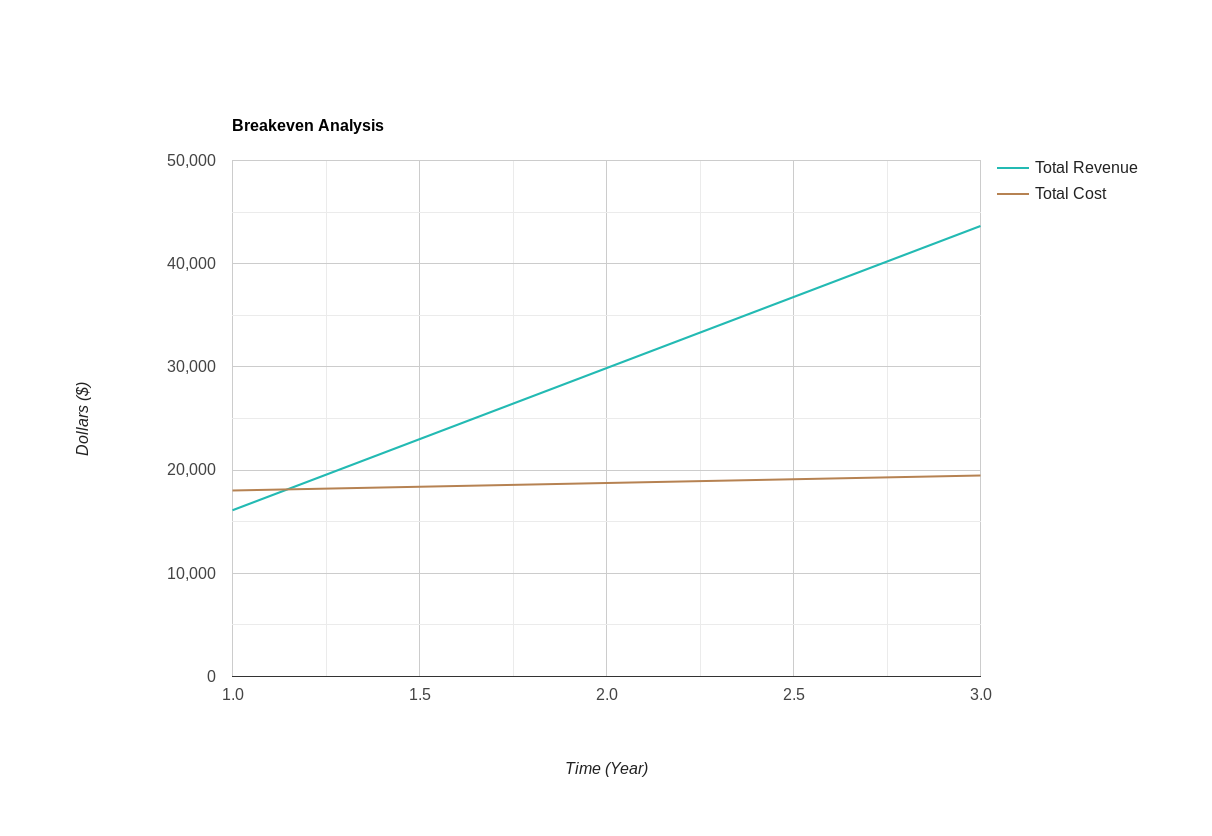
\includegraphics[width=\linewidth,height=15cm]{Diagrams/Breakeven.png}
    \caption{\small{Breakeven point calculation using graph.}}
  \label{fig:1}
\end{figure}
\par As seen from the graph the point at which the two lines intersect is when the time is equal to about 1.125 year,which is time needed for the business to breakeven and this is good and shows that the business is worth investing.
\section{Potential Marketshare}
The following tables shows the market share of the business for the first three years from its start.The market size is based on studies and statistics mentioned in these sites \url{https://www.wepc.com/news/video-game-statistics/} and \url{https://steamspy.com/genre/Indie}.
% Please add the following required packages to your document preamble:
% \usepackage[table,xcdraw]{xcolor}
% If you use beamer only pass "xcolor=table" option, i.e. \documentclass[xcolor=table]{beamer}
\begin{table}[!H]
\begin{tabular}{|l|l|l|l|}
\hline
\cellcolor[HTML]{23BAB3}\textbf{Market Opportunity in Revenue} & \multicolumn{3}{l|}{\textbf{\$4 M}}                                                                                         \\ \hline
                                                               & \cellcolor[HTML]{529BB6}\textbf{Year 1} & \cellcolor[HTML]{529BB6}\textbf{Year 2} & \cellcolor[HTML]{529BB6}\textbf{Year 3} \\ \hline
\cellcolor[HTML]{23BAB3}\textbf{Yearly Objective (Revenue)}    & \textbf{16000}                          & \textbf{28000}                          & \textbf{44000}                          \\ \hline
\cellcolor[HTML]{23BAB3}\textbf{Growth Rate}                   & \textbf{}                               & \textbf{175\%}                          & \textbf{157\%}                          \\ \hline
\cellcolor[HTML]{23BAB3}\textbf{Required Market Share}         & \textbf{0.4\%}                          & \textbf{0.7\%}                          & \textbf{1.1\%}                          \\ \hline
\end{tabular}
\end{table}

\end{document}
